\documentclass[a4paper,12pt]{extarticle}

\usepackage[utf8]{inputenc}
\usepackage[francais]{babel}
\usepackage[T1]{fontenc}
\usepackage[pdftex]{graphicx}
\usepackage{url}
\usepackage{caption}
\usepackage{graphicx}
\usepackage{multirow}
\usepackage{fancyhdr}

\pagestyle{fancy}

\setlength{\parindent}{0cm}
\setlength{\parskip}{1ex plus 0.5ex minus 0.2ex}

\newcommand{\hsp}{\hspace{20pt}}
\newcommand{\HRule}{\rule{\linewidth}{0.5mm}}
\renewcommand{\headrulewidth}{1pt}
\renewcommand{\footrulewidth}{1pt}

\fancyhead[L]{\leftmark}
\fancyhead[R]{}
\fancyfoot[C]{\textbf{page \thepage}} 
%opening

\begin{document}
	\begin{titlepage}
		\begin{sffamily}
		\begin{center}
		% Upper part of the page. The '~' is needed because \\
		% only works if a paragraph has started.
		%\includegraphics[scale=1]{univangers.jpg}~\\[1.5cm]
		
		
\includegraphics[scale=0.5]{Img/logo/logo_iutangers}~\\[1.5cm]
		
		\textsc{\LARGE Université d'Angers}\\[1.5cm]
		
		% Title
		\HRule \\[0.4cm]
		{ \huge \bfseries Stage en entreprise}{\bfseries  \\[0.4cm]}
		\HRule \\[1.5cm]
		
		% Image
		\begin{center}
			
\includegraphics[scale=1]{Img/logo/logo_fleurymichon}
		\end{center}
		
		\textsc{\LARGE Logiciel de communication entre un système MES et des équipements industriels.}\\[2cm] 
		
		% Author and supervisor
		\begin{minipage}{0.4\textwidth}
			\begin{flushleft} \large
				FRESNEAU \textsc{Quentin}
			\end{flushleft}
		\end{minipage}
		
		\vfill
		\HRule\\[2cm]
		% Bottom of the page
		{\large 26 Avril 2017}
		
		\end{center}
		\end{sffamily}
	\end{titlepage}
	\clearpage
	
	\tableofcontents
	\clearpage

	\section{Remerciements}
		\paragraph{}

	Je tiens à remercier dans un premier temps, toute l’équipe pédagogique de la faculté des sciences d’Angers et les intervenants professionnels responsables de la formation licence professionnelle Logiciel Libre pour avoir assuré la partie théorique de celle-ci.\\
Je remercie également Monsieur Jean-Philippe Hamiez pour l’aide, les conseils et les réponses à mes questions concernant les missions évoquées dans ce rapport, qu’il m’a apporté lors des différents suivis.\\
Je tiens à remercier tout particulièrement et à témoigner toute ma reconnaissance aux personnes suivantes, pour l’expérience enrichissante et pleine d’intérêt qu’elles m’ont fait vivre durant ces quatre derniers mois de stage au sein de l’entreprise Fleury Michon : \\
Monsieur Deschamps Stéphane, Responsable de projet informatique, mon tuteur, pour m’avoir intégré rapidement au sein de l’entreprise et m’avoir accordé toute sa confiance ; pour le temps qu’il m’a consacré tout au long de cette période, sachant répondre à toutes mes interrogations ; sans oublier sa participation au cheminement de ce rapport, Monsieur Boisseau Jérôme, Responsable de projet informatique, pour son accueil et son aide pour les quelques questions que j’ai pu lui poser durant la période de stage, Messieurs Guilloteau Kevin, Réau Pierrick, Marais Stéphane et Fabien Ribereau avec qui j’ai travaillé pour mettre en place le projet.\\
Enfin, j’aimerais terminer par remercier l’ensemble du personnel informatique du site de Pouzauges et de Chantonnay de Fleury Michon pour leur accueil sympathique et leur coopération professionnelle tout au long de ces quatre mois.\\

	\clearpage
	
	\section{Introduction}
		\paragraph{}

	Dans le cursus de formation de la Licence Professionnelle Logiciel Libre, le stage est conçu comme un processus d’immersion réelle dans la vie professionnelle dans le domaine de l’informatique. Celui-ci complète les six mois de formation théorique par un stage en entreprise de 18 semaines du 01 avril 2017 au 31 juillet 2017.
J’ai donc choisi d’effectuer mon stage au sein du service informatique de l’entreprise Fleury Michon à Pouzauges.\\
Au cours de ce stage, je n’ai pas effectué une seule mission principale mais un ensemble de tâches ayant attrait à différentes compétences que pourrait exiger le métier de développeur informatique ou d’analyste programmeur. En quoi consistent mes missions ? Quelles sont leurs utilités pour l’entreprise ?\\
Ce rapport, après une présentation de l’entreprise en première partie, explicitera les différentes tâches que j’ai effectuées, puis démontrera leur utilité en les positionnant au cœur du fonctionnement courant de l’entreprise.\\

	\clearpage
	
	\section{Présentation de l’entreprise}
	
	\subsection{Historique du groupe}
		\paragraph{}

	L’Histoire de Fleury Michon commence à partir de 1905, Félix Fleury s'associe à Lucien Michon, son beau-frère négociant en viande, tous les deux d’origines vendéennes. Ils déposent ensemble les premiers statuts juridiques des établissements Fleury \& Michon.\\
    La période entre 1905 et 1950 correspond aux fondations du groupe. En effet, les fondations du groupe commencent par l’installation des différents bâtiments (notamment Pouzauges en 1934) mais aussi par les modifications des recettes (avec une innovation dans la cuisson du jambon en 1954).
Puis les années 1960 à 1970 marquent l’arrivée des produits du groupe sur les grandes surfaces avec différentes gammes de produits de charcuterie mais aussi des plats cuisinés.\\
	Viens ensuite la période entre 1990 et 2000 qui est marquée par le développement de la notoriété de la société. En effet, avec entre autres l’arrivée du surimi et donc d’un nouveau marché pour l’entreprise mais aussi le développement dans le marché du catering et des plateaux-repas (restauration hors domicile). Cette période est aussi marquée par une reformulation des procédés de fabrication de tous les produits pour supprimer les additifs et limiter le sel et le gras. De plus, elle profite du développement de sa notoriété pour mettre l’accent sur la croissance de la marque et sur le développement à l'international. Ainsi, elle rachète le concurrent Olida, réalise un partenariat avec Beretta (en Italie) pour fonder Piatto Freschi Italia en 2002, et un autre avec Martinez Loriente (en Espagne) en 2005. Elle fait aussi l'acquisition de la société Delta Daily Food au Canada en 2006. Aujourd’hui, le groupe Fleury Michon possède 15 sites de production dont 7 à l'international.\\
    Enfin, depuis 2010, c’est l’engagement qui est mis en valeur par Fleury Michon avec la signature de la 1ère charte d’engagement nutritionnel PNNS (Programme National Nutrition Santé) et avec le lancement de la campagne \#VenezVérifier créée pour montrer aux consommateurs/blogueurs comment le surimi est produit de la pêche du poisson en Alaska jusqu'à leur préparation en Vendée sur le site de traiteur de la mer (TLM à Chantonnay).\\

	\clearpage

	\subsection{L’entreprise Fleury Michon}
		\paragraph{}

	L’entreprise Fleury Michon est une Société Anonyme (SA) à conseil d'administration. L’entreprise est composée de 15 sites de production regroupés dans 8 pays à travers le monde. L’ensemble de ces sites propose aujourd’hui un panel complet de produit fabriqué comme des plats cuisinés, du blanc de dinde (et poulet), du jambon, des ingrédients pour cuisine, des boxs, des produits tartinables, de la viande à poêler, des viandes rôties et cuisinées ainsi que du surimi.\\
Elle possède trois pôles d’activité qui sont :\\
	 - le pôle GMS libre-service en France (coeur du métier),\\
	- le pôle international,\\
	- le pôle ventes avec services.\\
Le pôle GMS correspond à la distribution en grande surface dans laquelle les clients visés sont des personnes de tous les jours. Le pôle international est lui aussi concerné par la distribution en grande surface mais aussi par le catering aérien (alimentation pour les trajets en avion). Enfin, le troisième pôle concerne les nouveaux services alimentaires c’est-à-dire la recherche de nouveaux circuits de distribution, mode d’achats ou encore de lieux de vente.\\
Le chiffre d’affaires de Fleury Michon (disposé à Pouzauges) atteint un peu plus de 39,6 millions d’Euros pour un capital social de 13 382 658 d’Euro. Le chiffre d’affaires consolidé du groupe Fleury Michon atteint 737,8 millions d’Euros.\\
L’entreprise de Pouzauges se divise en différents pôles : production, maintenance, informatique...etc.
Nous allons donc nous intéresser davantage au pôle informatique. Celui-ci regroupe une cinquantaine de personnes et est divisé en 5 pôles majeurs avec le pôle infrastructure, le pôle industriel, le pôle gestion, le pôle digital et le pôle services.\\

logo (a voir)
photo entreprise (a voir)

	\subsection{Situation géographique}
		\paragraph{}

	Le site de Fleury Michon (la Gare) est basé à Pouzauges au lieu-dit “La gare”, il correspond aussi au siège social de l’entreprise. Durant ma période de stage, j’ai été amené à travailler sur différents sites de production comme celui de Pouzauge (la Gare) lorsque j’étais en période d’analyse et de développement ou encore celui de Chantonnay (TLM)qui se situe dans la zone industrielle lorsque j’étais en phase de fin de développement et en phase de test et débogage.\\
Ces deux sites ont 20 km d’écarts et sont situés entre 15 et 20 km de mon domicile.\\

	\centerline{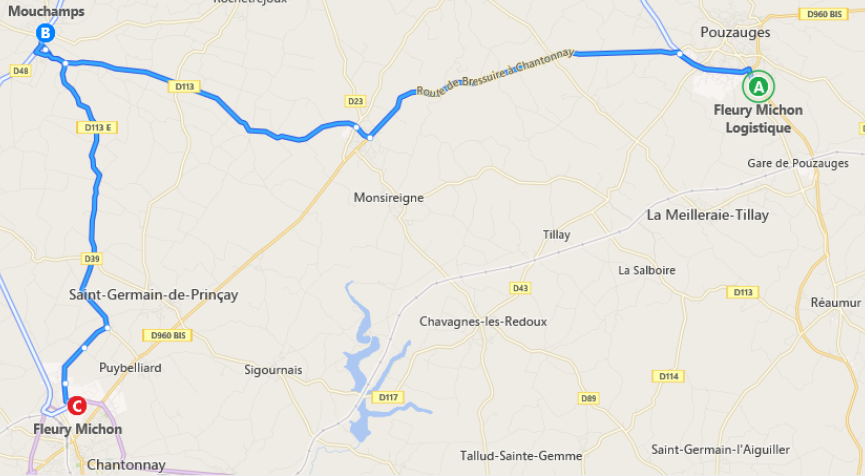
\includegraphics[scale=0.40]{Img/Img_SituationGeo}}

	\subsection{Présentation de l'équipe et des locaux}
		\paragraph{}

	Aujourd’hui, le service informatique comporte un peu plus de 50 personnes. Au cours de mon stage j’ai été mené à travailler avec certaines d’entre elles.
J’ai surtout travaillé en collaboration avec Deschamps Stéphane, Guilloteau Kevin, Réau Pierrick, Marais Sébastien, Clairet Arnaud, Bibard Nicolas et Ribereau Fabien pour mener à bien ce projet.\\

	\clearpage
	
	\section{Présentation du projet de stage}
	
	\subsection{Analyse du besoin}
		\paragraph{}


	Sur le site de production de Chantonnay (TLM - Traiteur de La Mer) se fait fabriquer l’un des produits que l’entreprise propose : le surimi.
Au suivi des nombreux processus de cuisson, mise en barquette, pasteurisation… le dernier de cette chaîne est celle du suremballage. Sur celle-ci, un automate est chargé de communiquer avec deux étiqueteuses de la marque VideoJet afin de pouvoir étiqueter l’ensemble des cartons qui compose les palettes arrivant sur le tapis. Ce système est dirigé par un utilisateur qui lance l’étiquetage via un poste.\\
Sur ce poste est installé l’application MesToColis qui est chargée de communiquer les informations nécessaires à l’étiquetage tel que la DLC du produit, le numéro de lot, le nom du produit, la liste des allergènes… Le système existant proposait à l’utilisateur un seul choix d’envoi des données, l’entreprise avait décidé de sous-traiter cet envoi de données via un petit applicatif nommé iDaro qui lisait un dossier lors de l’envoi des données. Ce dossier devait alors contenir un masque d’étiquette qui comprenait les informations nécessaires à l’étiquetage. Ce système fonctionnant sur la ligne 98 du site de production, l’entreprise a souhaité l’implanter sur la ligne 99 mais des problèmes de réinstallation du logiciel iDaro sur un autre serveur faisaient leur apparition. Suite à ça, une autre étiqueteuse a fait son entrée dans le système (appelé “Mulet”) qui était utilisé uniquement lorsqu’une étiqueteuse n’avait pas correctement étiqueté certains cartons.\\
Au bout de quelques années, l’entreprise qui sous-traitait cet échange de données n’était plus joignable et pour des raisons évidentes de sécurité et d’indépendance, Fleury Michon a choisi de redévelopper cet échange de données au sein de l’application existante. A la suite d’une réunion, rassemblant les concerner par le projet, lors de la première semaine de mon stage, le but précis et certains choix ont été réalisés.\\

	\clearpage

	\subsection{But du projet}
		\paragraph{}

	Le but du projet est donc de supprimer le logiciel iDaro. Pour cela, l’entreprise propose donc de développer en interne à l’application MesToColis, l’échange de données vers soit un automate (ou plusieurs) soit une étiqueteuse (ou plusieurs). L’échange entre le MES et une étiqueteuse a été géré en 2017 par Pierrick Réau avec l’utilisation du protocole Zipher (fourni par le fournisseur des étiqueteuses), il est donc réutilisable à l’avenir. Sur la ligne L98 de TLM, deux étiqueteuses VideoJet ainsi que le Mulet sont gérées par un seul automate de la marque Schneider Electronics. Celui-ci est chargé de communiquer les informations présentes dans le masque d’étiquette ainsi que les informations reçues par l’automate de palettisation aux deux étiqueteuses pour qu’elles puissent étiqueter convenablement la palette qui arrive sur le tapis. Les informations sont de deux types, celles qui concernent les informations du produit comme la DLC (Date Limite de Consommation), le libellé et le code du produit… (etc) et celles qui concernent les informations du portail Jyga c’est-à-dire tous les paramètres que les étiqueteuses doivent prendre en compte comme le nombre de couche de cartons sur la palette, le nombre total de cartons à étiqueter... (etc) pour mener à bien l’étiquetage des colis.\\
La communication entre l’automate et le logiciel MES a été fait avec le protocole OPC. La suite de la communication entre l’automate et les étiqueteuses a été fait par M. Marais Sébastien, responsable maintenance automate, via le protocole Zipher ASCII.

	\clearpage
	
	\section{Élaboration du projet}
	
	\subsection{Partage du travail}
		\paragraph{}

	Etant en entreprise, le travail effectué n’a pas vraiment été partagé puisque le projet m’était destiné. En revanche, j’ai travaillé avec plusieurs personnes pour pouvoir avancer dans le projet lorsque j’étais face à des difficultés. Dans le cadre du développement de l’application MesToColis pour le site TLM à Chantonnay, je me suis occupé de la moitié de la communication entre le logiciel MES et l’automate avec l’envoi de données et M. Sébastien Marais s’est occupé de l’autre moitié de la communication entre l’automate et les étiqueteuses.\\ \\
	
			\centerline{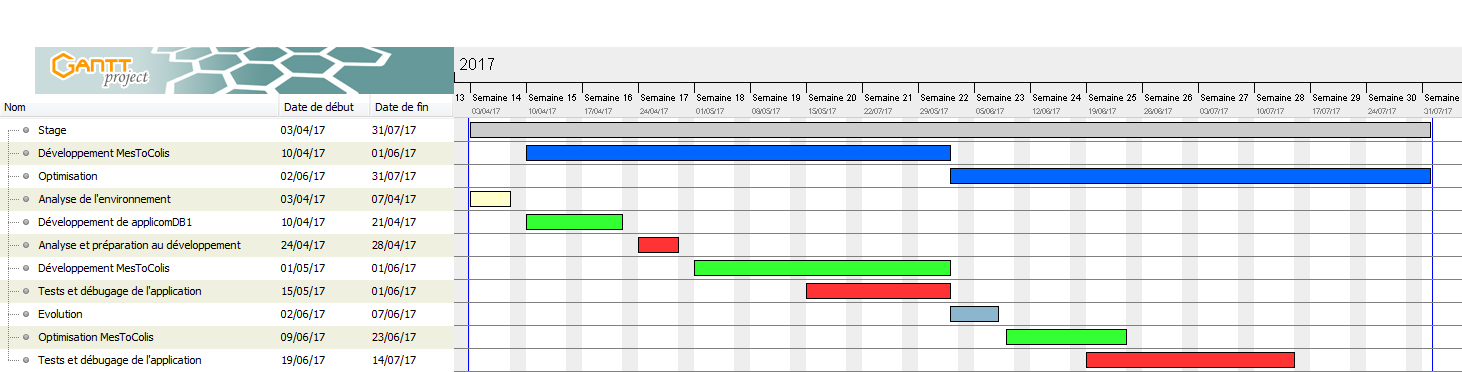
\includegraphics[scale=0.4]{DiagrammeDeGantt}}
	
	\subsection{Matériel mis à disposition}
		\paragraph{}
			
	Ordinateur ThinkPad (intel inside, Core i5).\\
Automate Schneider M340 avec afficheur pour les tests.\\
	
	\subsection{Réalisation hors rapport}
		\paragraph{}

	En marge de ce rapport, il a aussi fallu que je rédige une spécification détaillée sur le nouveau fonctionnement de l’application MesToColis pour que l'existant puisse être repris par une autre personne. Cette documentation a été ajouté au sein de l’intranet de l’entreprise.
Pour faciliter la rédaction du rapport de stage, j’ai utilisé Google Drive pour modifier le plus facilement et rapidement possible le contenu du rapport.\\
J’ai aussi mis en place un GIT dans lequel je m’étais à jour chaque semaine un journal de bord et un descriptif des problèmes rencontrés (et de leurs solutions) pendant toute la période du stage mais aussi pour y stocker les différents fichiers utiles à l’élaboration du rapport. J’y ai aussi mis un diagramme de Gantt dans lequel je faisais apparaître les tâches du projet et le temps passé sur chacune d'elles.\\
GIT du projet : \url{https://github.com/qfresneau/Stage}\\

	\section{Développement}
		\paragraph{}
			à voir\\
	\clearpage
	
	\section{État final du projet}
		\paragraph{}
			à voir\\
	\clearpage
	
	\section{Conclusion}
		\paragraph{}
			à voir\\
	\clearpage
	
	\section{Sources}
		\paragraph{}
			à voir\\
	
	\section{Glossaire}
		\paragraph{}
			à voir\\
	\clearpage
	
	\section{Annexes}
		\begin{center}	\centerline{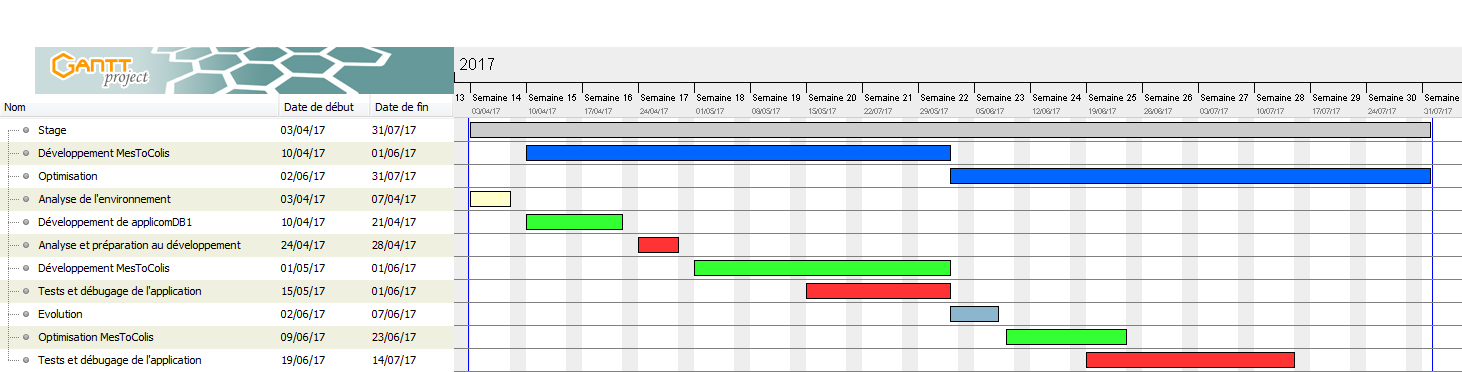
\includegraphics[scale=0.35,angle=270]{DiagrammeDeGantt}}
		\end{center}

\end{document}
\newline